        \clearpage
        \begin{figure*}[ht]
            \pdfbookmark[2]{ID 06}{figure_id_06}
        	\centering
            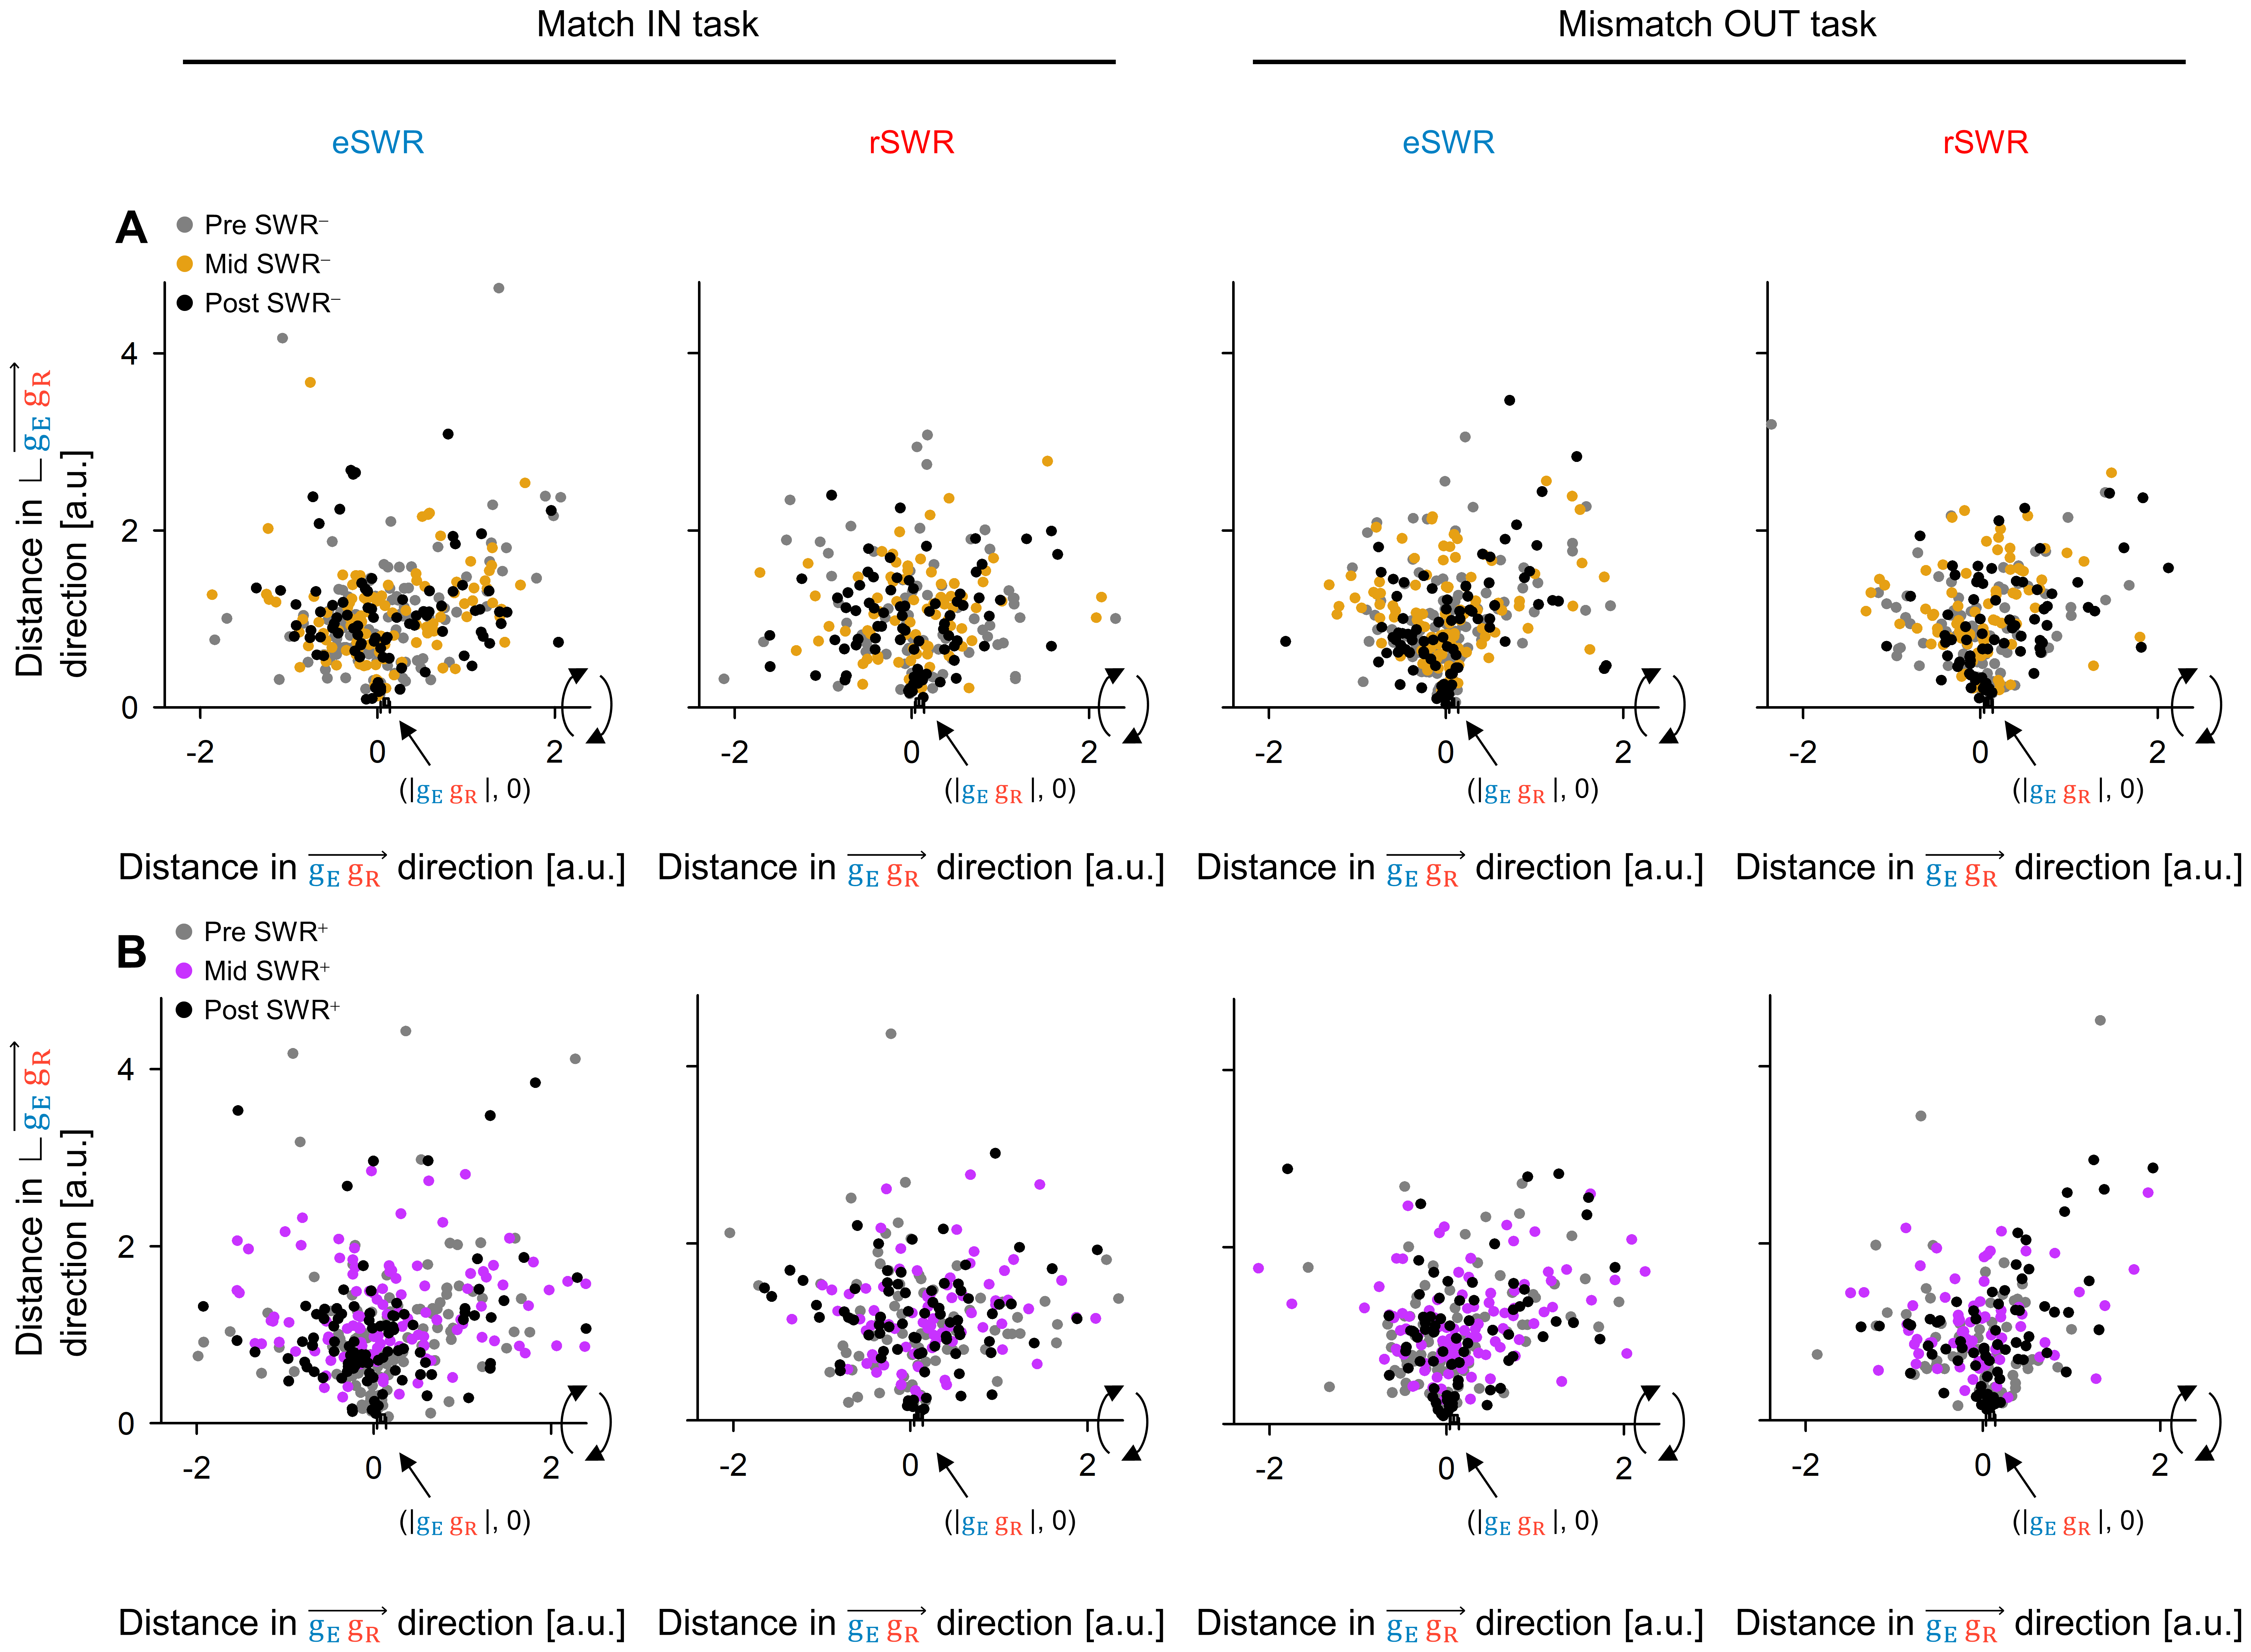
\includegraphics[width=1\textwidth]{./src/figures/png/Figure_ID_06.png}
        	\caption{\textbf{
Visualization of Neural Trajectory During SWR in Two-Dimensional Space
}
\smallskip
\\
The panels depict hippocampal neural trajectories (NTs) during SWR projected onto two-dimensional spaces. \textbf{\textit{A.}} Shows the hippocampal NTs as point clouds during pre-SWR$^-$ (\textit{gray}), mid-SWR$^-$ (\textit{yellow}), and post-SWR$^-$ (\textit{black}). \textbf{\textit{B.}} Conveys the equivalent for SWR$^+$ rather than SWR$^-$. The projection was executed as follows: First, a linear transformation placed $\mathrm{g_{E}}$ at the origin $O$ (0,0), and $\mathrm{g_{R}}$ at ($\lVert \mathrm{g_{E}g_{R}} \rVert$, 0). The point cloud was subsequently rotated around the $\mathrm{g_{E}g_{R}}$ axis (similar to the x axis) for adaptation to two-dimensional spaces. Thus, within these two-dimensional spaces, the distances from point $O$ and the angles for the $\mathrm{g_{E}g_{R}}$ axis are retained as in the original three-dimensional spaces created by GPFA. Abbreviations: SWR denotes sharp-wave ripple events; eSWR refers to SWR during the encoding phase; rSWR signals SWR during the retrieval phase; SWR$^+$, characterizes an SWR event; SWR$^-$ signifies control events for SWR$^+$; pre-SWR, mid-SWR, or post-SWR, represent the time intervals from $-800$ to $-250$ ms, from $-250$ to $+250$ ms, or from $+250$ to $+800$ ms from the center of the SWR.
}
% width=1\textwidth
        	\label{fig:06}
        \end{figure*}
